\documentclass[10pt, czech]{beamer}
\usepackage[czech]{babel}
\usepackage[utf8]{inputenc}
\usepackage{hyperref}
\usepackage{times}
\usepackage{algpseudocode}

\usetheme{Madrid} %Antibes

\title{Typografie a publikování -- projekt 5}
\subtitle{Prezentace}
\author{Ondřej Lukášek}
\institute[Vysoké učení technické v Brně]
{
  Vysoké učení technické v Brně, \\
  Fakulta informačních technologií
}
\date{\today}

\begin{document}

% SLIDE 1
\begin{frame}
    \titlepage
\end{frame}

% SLIDE 2
\begin{frame}{Obsah prezentace}
    \tableofcontents
\end{frame}

% SLIDE 3
\section{Úvod}
\begin{frame}{Úvod -- BFS}
    \begin{block}{Přeložení pojmu}
        BFS znamená \textit{Breadth-first search} (vyhledávání do šířky).
    \end{block}
    \begin{itemize}
        \item Vynalezena roku 1945 (Konrad Zuse) -- disertační práce.
        \item Publikována až roku 1972.
        \item Hojně využívaná v prohledávání binárních stromů.
        \item Pokud cílový stav existuje, metoda ho vždy nalezne.
    \end{itemize}
\end{frame}

% SLIDE 4
\section{Podrobnější popis}
\begin{frame}{Podrobnější popis}
    \begin{itemize}
        \item Vstupem je graf $G = (V, E)$ a vrchol $s \in V$.
        \item Vstupní graf může být jak orientovaný, tak i neorientovaný.
        Následně se prochází všechny vrcholy dostupné z $s$ a počítá se počet hran z $s$.
    \end{itemize}
    \begin{alertblock}{Důležité informace}
        Metoda vytváří strom prohledávání do šířky s kořenem $s$ obsahující všechny vrcholy dosažitelné z $s$. Cesta z~$s$ do~$v$ je nekratší cestou v~grafu.
    \end{alertblock}
    \begin{itemize}
        \item Při průcodech se vrcholy obarvují černou, šedou a bílou barvou.
        \item Nejvhodnější reprezentace přes seznam sousedů.
    \end{itemize}
\end{frame}

% SLIDE 5
\section{Pseudokód}
\begin{frame}{Pseudokód -- 1/2}
    \begin{algorithmic}[1]
        \State $color[s] \gets GREY$
        \State $d[s] \gets 0$
        \State $\pi[s] \gets NIL$
        \For{$\textsc{každý vrchol} \ u \in V - \{s\}$}
            \State $color[u] \gets WHITE$
            \State $d[u] \gets \infty$
            \State $\pi[u] \gets NIL$
        \EndFor
        \State $\textsc{InitQueue}(Q)$
        \State $\textsc{Add}(Q, s)$
        \While{$\textsc{not IsEmpty}(Q)$}
            \State $u \gets \textsc{Front}(Q)$
            \State \textbf{viz následující slide}
            \State $\textsc{Remove}(Q)$
            \State $color[u] \gets BLACK$
        \EndWhile
    \end{algorithmic}
\end{frame}

% SLIDE 6
\begin{frame}{Pseudokód -- 2/2}
    Následující kód vložte do 13 řádku přechozího slidu:
    \bigskip
    \begin{algorithmic}[1]
        \For{$\textsc{každý} \ v \in Adj[u]$}
            \If{$color[v] = WHITE$}
                \State $color[v] \gets GREY$
                \State $d[v] \gets d[u]+1$
                \State $\pi[v] \gets u$
                \State $\textsc{Add}(Q, v)$
            \EndIf
        \EndFor
    \end{algorithmic}
    \medskip
    \begin{itemize}
        \item $color[u] \in$ {WHITE, GRAY, BLACK}.
        \item $\pi[u]$ je předchůdcem $u$ na cestě z $s$.
        \item $d[u]$ je počet hran $u$ od $s$
    \end{itemize}
\end{frame}

% SLIDE 7
\section{Příklad algoritmu}
\begin{frame}{Příklad algoritmu}
    \begin{Example}
        \begin{itemize}
            \item Mějme graf o 8 vrcholech.
            \item Startovacím vrcholem je $s$.
            \item Ostatními vrcholy jsou:\\
                $a, b, c, d, e, f, g$
            \item Nastavíme pořadí návštěv u všech prvků na $\infty$, kromě $s$, který je               startovacím prvkem, tedy bude mít hodnotu $0$.
        \end{itemize}
    \end{Example}

    \begin{block}{Poznámka}
        Pro lepší čitelnost si černou barvu nahradíme modrou barvou.
    \end{block}
\end{frame}

% SLIDE 8
\begin{frame}{Příklad algoritmu}
    \centering
    \only<1>{\scalebox{0.5}{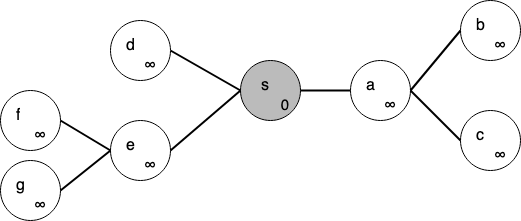
\includegraphics{img/priklad1.png}}}
    \only<2>{\scalebox{0.5}{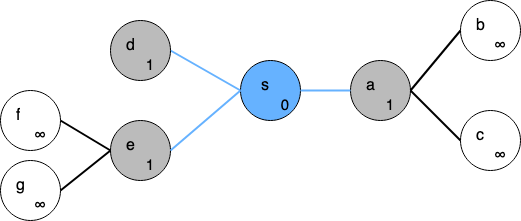
\includegraphics{img/priklad2.png}}}
    \only<3>{\scalebox{0.5}{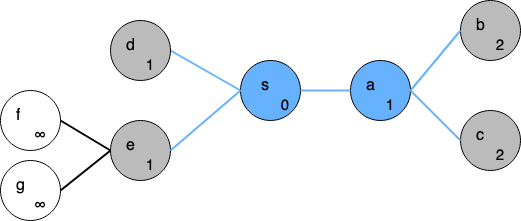
\includegraphics{img/priklad3.png}}}
    \only<4>{\scalebox{0.5}{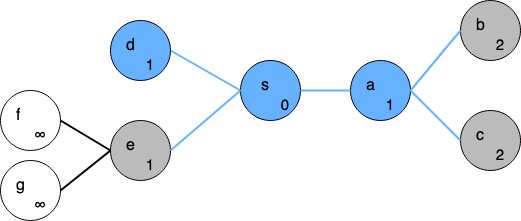
\includegraphics{img/priklad4.png}}}
    \only<5>{\scalebox{0.5}{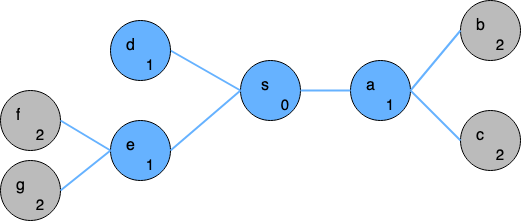
\includegraphics{img/priklad5.png}}}
    \only<6>{\scalebox{0.5}{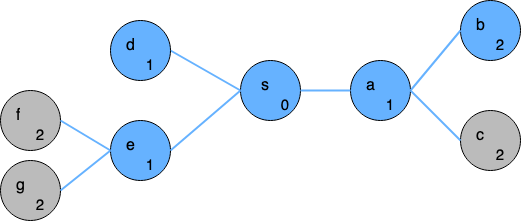
\includegraphics{img/priklad6.png}}}
    \only<7>{\scalebox{0.5}{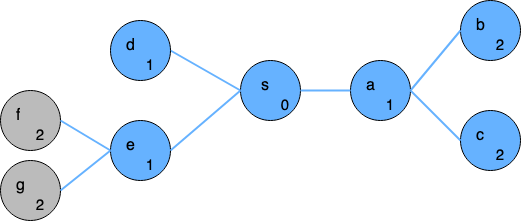
\includegraphics{img/priklad7.png}}}
    \only<8>{\scalebox{0.5}{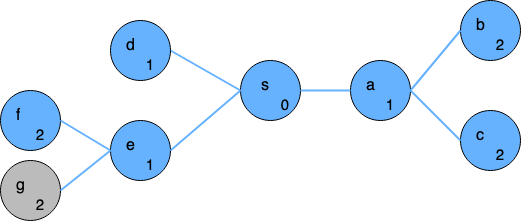
\includegraphics{img/priklad8.png}}}
    \only<9>{\scalebox{0.5}{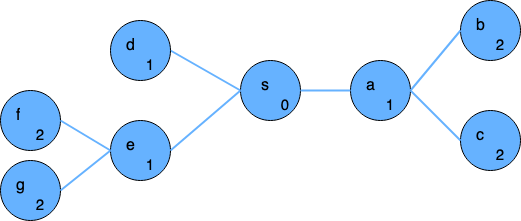
\includegraphics{img/priklad9.png}}}
    
\end{frame}

% SLIDE 9
\section{Složitost BFS}
\begin{frame}{Složitost BFS}
    \begin{itemize}
        \item Vkládání a vybírání prvku z fronty má konstantní složitost, tedy $O(1)$. Složitost pro $n$    prvků tedy bude $O(n)$.
        \item Protože se seznam, sousedů u každého vrcholu prochází pouze při jeho vybírání z fronty, seznam se skenuje nanejvýš jednou.
        \item Protože je suma délek těchto seznamů rovna $\Theta (m)$, je celkový čas skenování seznamu sousedů $O(m)$.
        \item Incializace trvá dobu $O(n)$.
    \end{itemize}
    \begin{alertblock}{Celková složitost}
        Celkový čas algoritmu je tedy $O(m+n)$.
    \end{alertblock}
\end{frame}

\begin{frame}{Zdroje}
    \begin{itemize}
        \item \url{https://moodle.vut.cz/mod/folder/view.php?id=223249}
        \item \url{https://www.geeksforgeeks.org/breadth-first-search-or-bfs-for-a-graph/}
        \item \url{https://moodle.vut.cz/mod/folder/view.php?id=288551}
    \end{itemize}
\end{frame}

\end{document}
